\subsection{Least Response Time Load Balancing Implementation}
% got 2,5 pages
With these experiments the goal is to better understand how the implementation details of the load balancing solution affect overall performance.
The previously performed initial evaluation revealed some potentially counter-intuitive behaviour, so to better inform our proposed implementation these experiments evaluate different implementation patterns.

An implementation of least response time load balancing is split in two parts: The gathering of response time data, and the conversion of that data into load balancing decisions.
As we discussed in our approach, we convert the response time data into weights, which are used as inputs to a weighted round robin load balancing implementation that ultimately makes load balancing decisions.
\subsubsection{Setup}
With these experiments our focus lies on these implementations of weighted round robin.
In particular we evaluate four different implementations of weighted round robin:
\begin{itemize}
    \item \textbf{Random:} this implementation uses a simple weighted random distribution. It is used as a baseline to compare other implementations to
    \item \textbf{Classic:} this represents the implementation used in the initial evaluation experiment\cite{wrr-kblinux}. It is deterministic and works through upstreams starting with the ones with the highest weight.
    \item \textbf{Adapted Classic:} an adaptation from the classic implementation, which allows for weights to be updated on the fly without the algorithm having to be restarted.
    \item \textbf{Smooth:} the implementation described in our approach and also used by nginx\cite{nginx-wrr}. It too is deterministic but alternates between upstreams with high and low weights in load balancing decisions.
\end{itemize}

We simulate a least response time load balancer with each of these implementations with 500 upstreams, which are simplified to sample response times from a lognormal distribution, over a timeframe of 500 seconds with a request rate of 5\gls{rps}.
Weights are updated every 15 seconds, except for the smooth weighted round robin implementation which is updated every second, since this is a core benefit afforded by the implementation we want to test explicitly.
The weight range for each implementation is [0;10] and response times get mapped linearly, i.e. using a scaling factor of 1.

\subsubsection{Results}

\begin{figure}
    \centering
    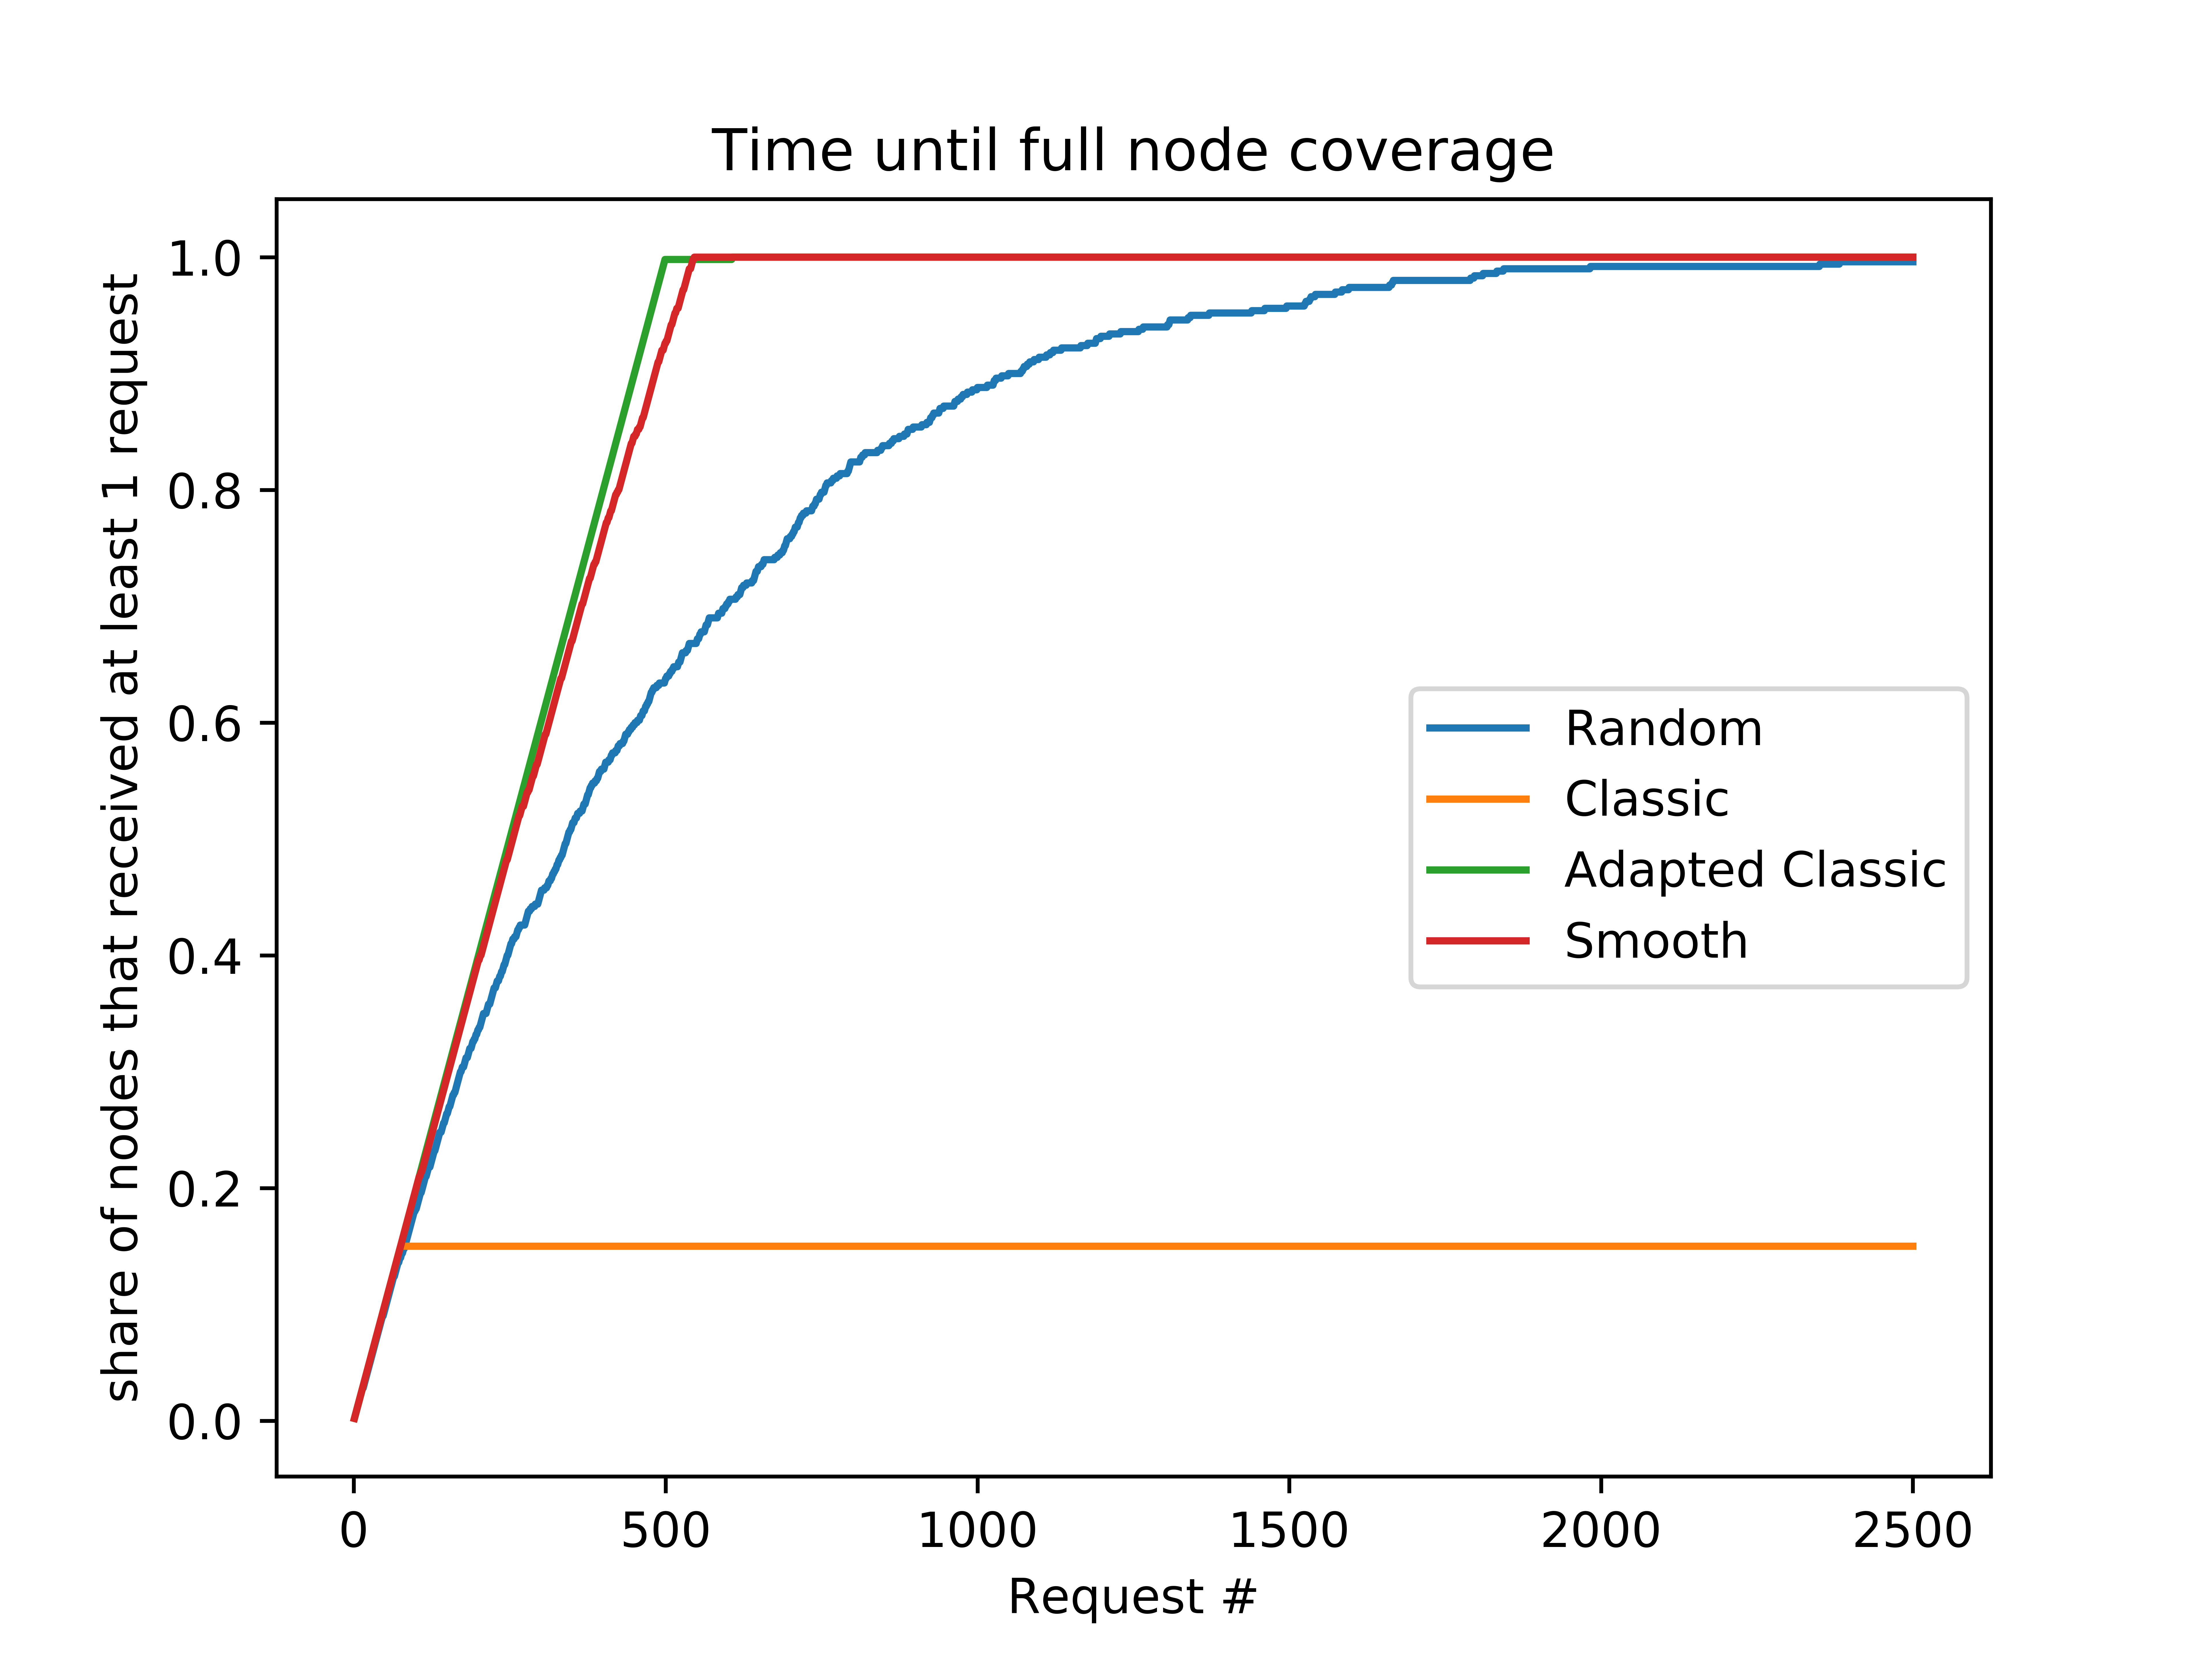
\includegraphics[width=11cm]{graphics/graphs/lb_imp_upstream_coverage.png}
    \caption{A graph showing how quickly each upstream receives at least one request with different weighted round robin implementations for least response time load balancing}
    \label{fig:lb_imp_upstream_coverage}
\end{figure}

\begin{figure}
    \centering
    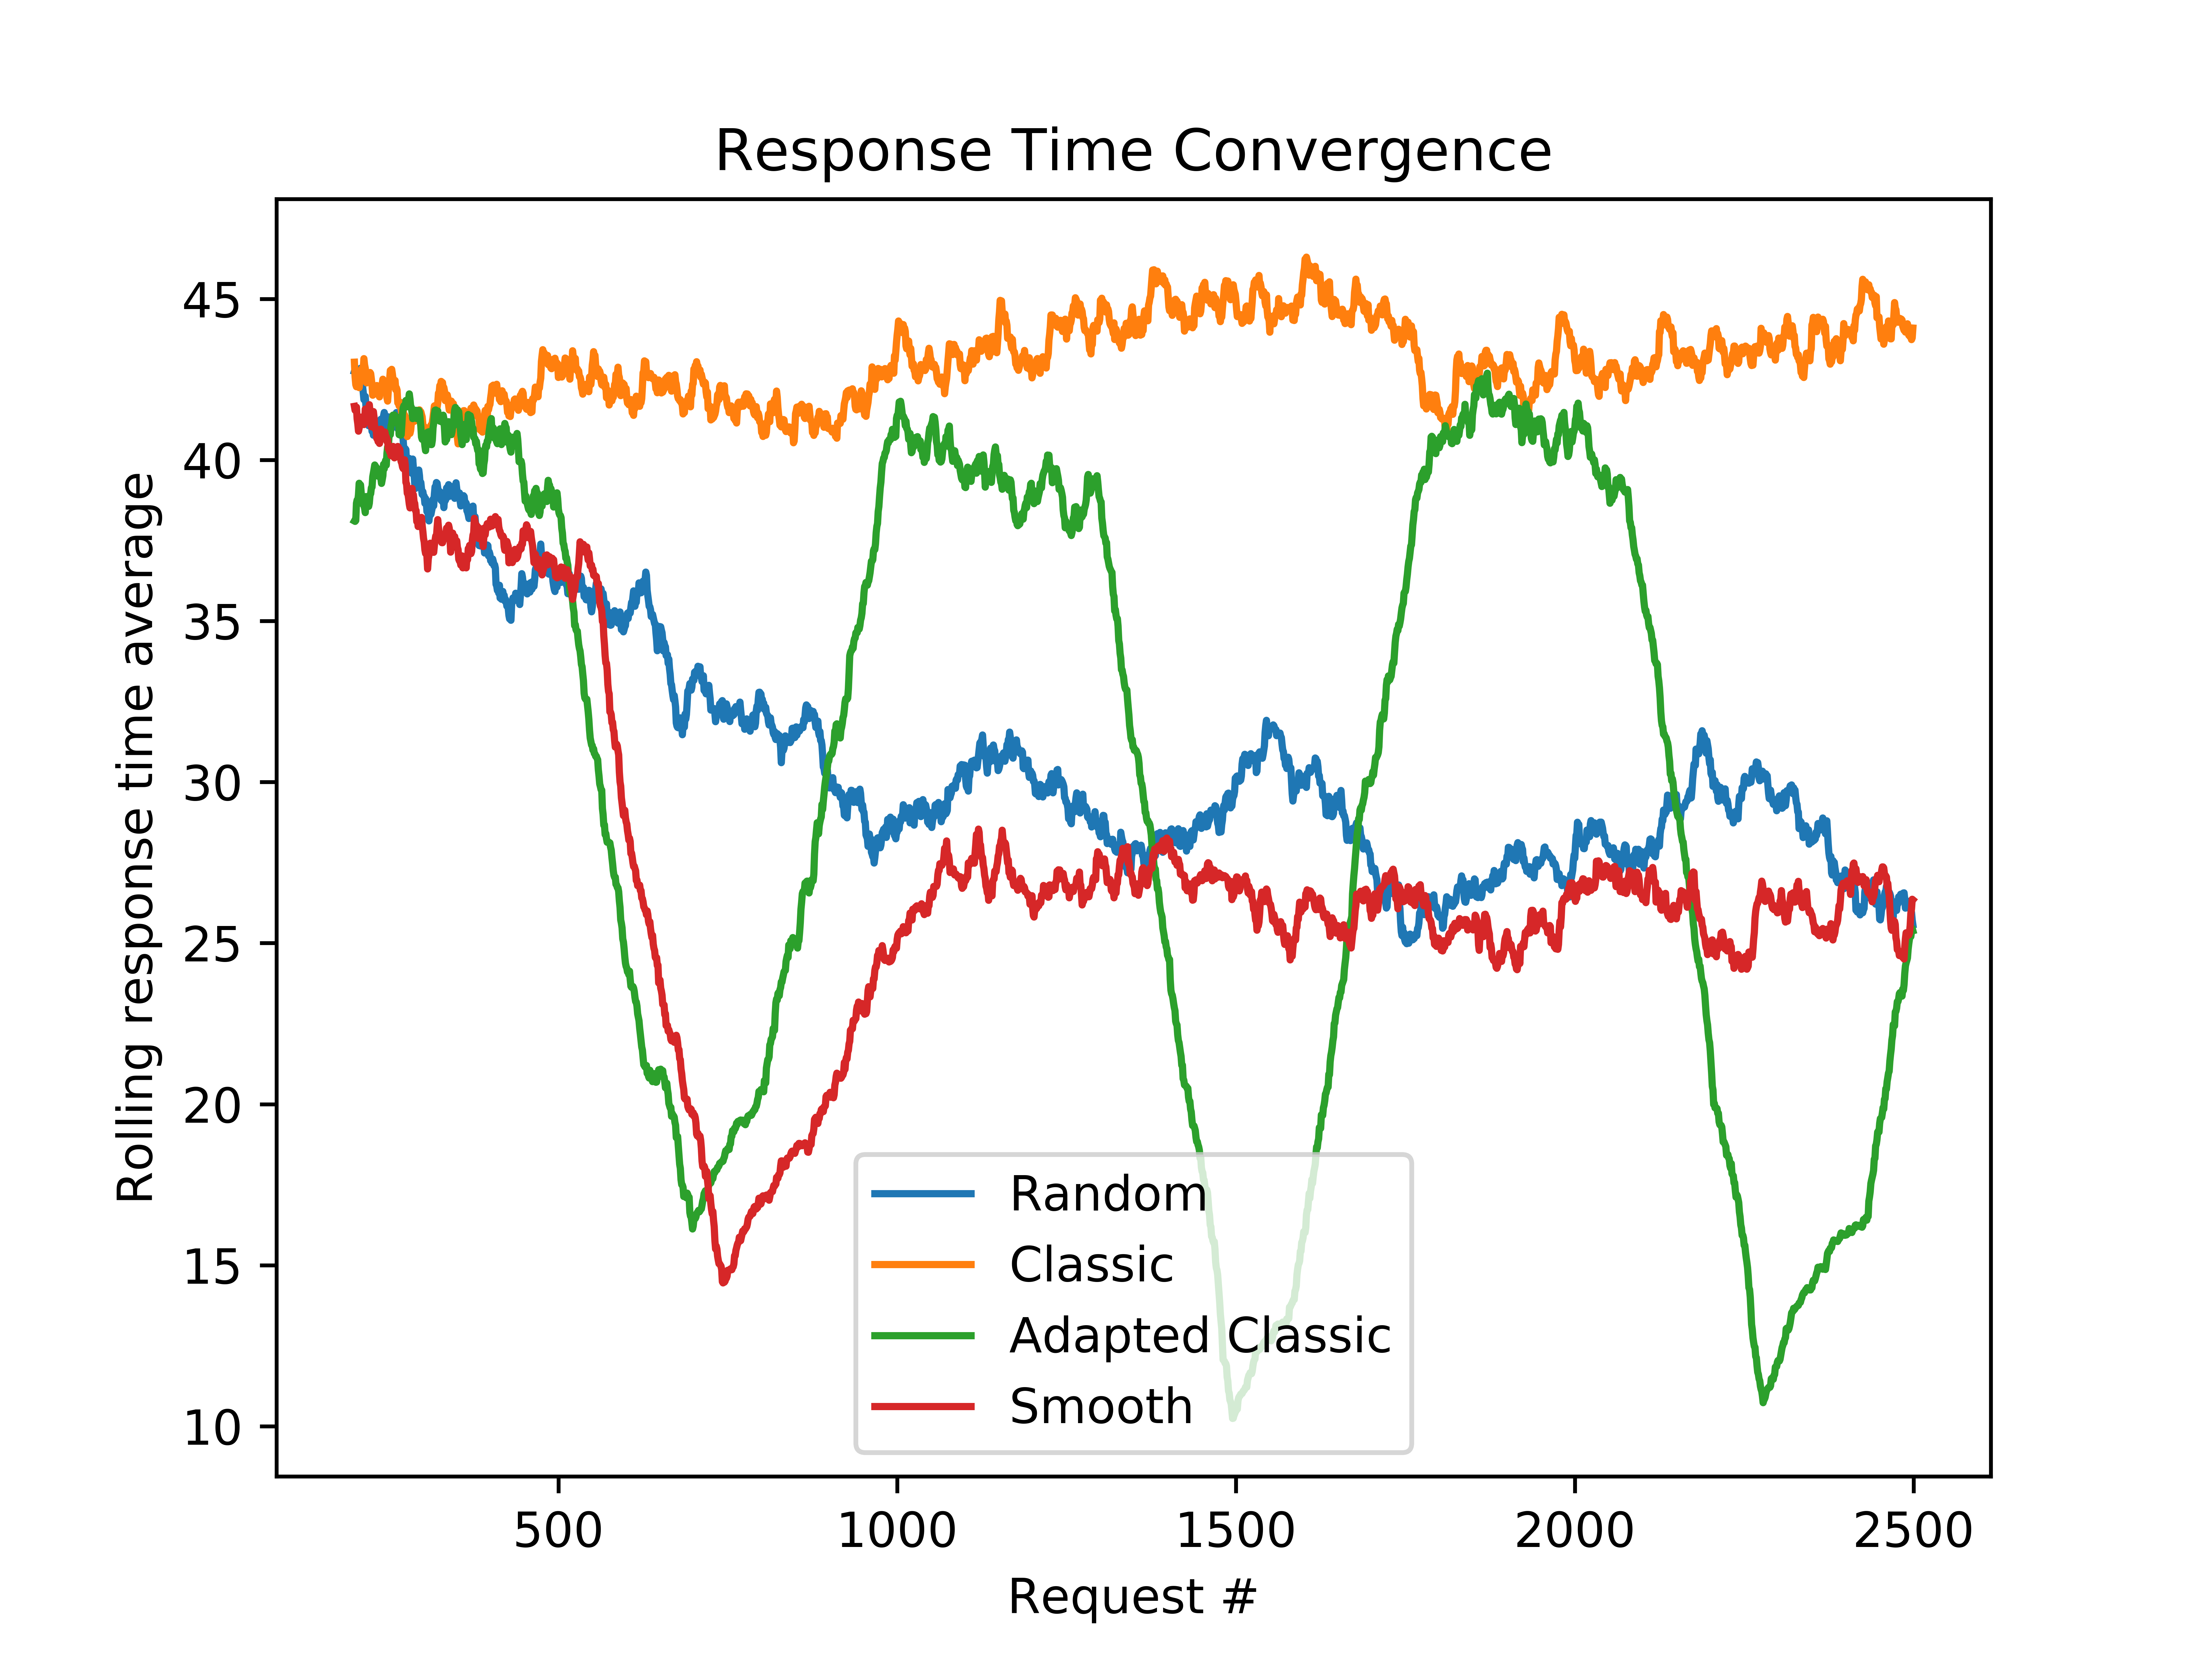
\includegraphics[width=11cm]{graphics/graphs/lb_imp_trt_convergence.png}
    \caption{Graph showing average response times converging for different weighted round robin implementations with least response time load balancing}
    \label{fig:lb_imp_rt_convergence}
\end{figure}

In our results we can see significant differences between the implementations.
First, as can be seen in Figure \ref{fig:lb_imp_upstream_coverage}, there are significant differences on how fast, or whether at all, every node in the system receives at least one request.
Since least response time load balancing relies on requests to evaluate the performance of an upstream, the quality of the solution is limited by the amount of information available about the upstreams.
We can see that the classic implementation never sends requests to more than a small subset of upstreams, which is due to its internal state being reset on weight updates.
While the random sampling eventually converges toward covering all upstreams, both the smooth and adapted classic implementation do so much more quickly.
The adapted classic is even a slight bit faster than the smooth implementation, but from our point of view we consider this difference to be negligible.

We also observe drastically different behaviour of the average response times between the different implementations.
Figure \ref{fig:lb_imp_rt_convergence} shows that Classic never reaches the level of performance of the other implementations, most likely due to it never discovering the faster subset of upstreams.
While we can also observe that for both the smooth and the random reference implementation average response times stabilize eventually, the adapted classic shows an alternating pattern of fast and slow response time averages.
This is due to the implementation, which works through the highest weighted upstreams first, before including the next highest weighted ones and so on.
Since the order in which this happens is deterministic this oscillating performance pattern forms.
The classic implementation shows the same behaviour, but due to it only ever sending requests to a smaller set of upstreams the pattern isn't as easily visible.
Note that as we are considering response time averages low values on the y-axis in Figure \ref{fig:lb_imp_rt_convergence} are desirable.












% for discussion: shows that default implementations don't necessarily fit least response time / edge computing and need to be adapted. Also shows how unintuitive behaviour can be
% can discuss potential performance tradeoffs between spending "resources" on node discovery vs. using already known nodes that work well.













